\documentclass[11pt,conference]{IEEEtran}
\usepackage[utf8]{inputenc}
\usepackage{amsmath}
\usepackage{amsfonts}
\usepackage{amssymb}
\usepackage{url}
\usepackage{graphicx}

\author{\IEEEauthorblockN{Andrew Rosen \qquad Brendan Benshoof \qquad Robert W. Harrison \qquad Anu G. Bourgeois}
    \IEEEauthorblockA{Department of Computer Science\\
        Georgia State University\\
        Atlanta, Georgia\\
        rosen@cs.gsu.edu \qquad  bbenshoof@cs.gsu.edu  \qquad rwh@cs.gsu.edu \qquad anu@cs.gsu.edu }
}
\title{The Sybil Attack on Peer-to-Peer Networks From the Attacker's Perspective}   % Or The Attacker's View of The Sybil Attack
\hyphenation{op-tical net-works semi-conduc-tor Chord-Reduce Map-Reduce Data-Nodes Name-Nodes}

\begin{document}

\maketitle


%TODO BETTER GRAPH
%TODO ATTACKER PRONOUNS

\begin{abstract}
This paper examines the amount of computation power required to perform an Eclipse attack on a P2P network.
%This paper explores the feasibility of performing naive Sybil attacks on a P2P network that completely occlude healthy nodes from each other.
The vulnerability of Distributed Hash Tables to Sybil attacks and Eclipse attacks has been well known for some time.
Most theoretical analyses of these attacks assume that the attacker is all-knowing and globally powerful.
This paper proves that these are not necessary characteristics and that a less powerful adversary can perform a successful Eclipse attack, while still obeying the protocol.% assumptions for an adversary to have to perform a Sybil attack.
Our analysis and experiments show that an adversary with a small number of machines and limiting their port usage to just the ephemeral ports can easily compromise a P2P system and occlude the majority of the links.

We examine the amount of computational effort required to perform an Eclipse attack using only Sybil identities and without poisoning routing tables via false advertisement.
We do this by analyzing the amount of effort it takes for an attacker with a given number of IP addresses to choose a port to obtain a desired hash key, a process we call \emph{mashing}.
%Mashing requires no additional resources on the adversary's end.
Our results showed that an adversary with just 3 IP addresses could compromise 90\% of all connections in a Chord network with 5000 nodes.
While mashing can be used for malicious behavior, we also describe methods and applications for the technique that are beneficial for performing load balancing.
This provides the flexibility for any node to effortless shoulder additional work from bottleneck locations, if acting for the good of the network.
\end{abstract}

\begin{IEEEkeywords}
    Sybil Attack; Eclipse Attack; P2P Security; Security; Distributed Hash Tables; P2P networks
    
\end{IEEEkeywords}

\section{Introduction}
One of the key properties of structured peer-to-peer (P2P) systems is the lack of a centralized coordinator or authority.
P2P systems remove the vulnerability of a single point of failure and the susceptibility to a denial of service attack \cite{sybil}, but in doing so, open themselves up to new attacks.

Completely decentralized P2P systems are vulnerable to \textit{Eclipse attacks}, whereby an attacker completely occludes healthy nodes from one another.
This prevents them from communicating without being intercepted by the adversary.
Once an Eclipse attack has taken place the adversary can launch a variety of crippling attacks, such as incorrectly routing messages or returning malicious data \cite{srivatsa2004vulnerabilities}.

One way to accomplish this attack is to perform a \emph{Sybil attack} \cite{sybil}.
In a Sybil attack, the attacker masquerades as multiple nodes, effectively over-representing the attacker's presence in the network to maximize the number of links that can be established with healthy nodes.
If enough malicious nodes are injected into the system, the majority of the nodes will be occluded from one another, successfully performing an Eclipse attack.

This vulnerability is well known \cite{dhtsec}. 
Extensive research has been done assessing the damage an attacker can do after establishing themselves \cite{srivatsa2004vulnerabilities}.
%Especially when a hash value to assign neighbors
Little focus has been done on examining how the attacker can establish himself in the first place and precisely how easily the Sybil attack can be accomplished.

One method to generate node locations is to assign them at random.
A Sybil attack against this method is fairly straightforward; the attacker just assigns his own nodes at ``random'' locations.
A more sophisticated method to generate node locations would use a hash function of some unique characteristic of the node.
For example, a Distributed Hash Table could use a hash of the node's IP address and port number.
In this paper, we show that using a hash function provides no protection against a Sybil attack.

Our goal is to look at the Sybil attack from the perspective of an adversary executing the Sybil attack.
We did a formal analysis on the breadth and depth of the presence an adversary could establish on a structured P2P network.
%We also constructed simulations showing how an attacker could insert themselves into the network and proceed to incrementally inject malicious nodes in between normal members of the network, a process we call \textit{mashing}.
We also constructed simulations demonstrating the steps an attacker could follow to perform a Sybil attack.
Once the attacker has joined the network, they can proceed to incrementally inject malicious nodes directly in between members of the network, a process we call \textit{mashing}.

%Why am I doing this?
Sybil attacks represent a significant threat to the security of any distributed system.
Many of the analyses on Tor \cite{dingledine2004tor} emphasize the vulnerability of Tor to the Sybil attack \cite{bauer2007low}.
This threatens the anonymity of Tor users.

Sybil attacks are also a threat to P2P systems such as BitTorrent, which is essential to a wide variety of users.
BitTorrent is currently the \textit{de facto} platform for distributing large files scalably among tens of thousands of clients.
Many implementations rely on Mainline DHT (MLDHT) \cite{mainline} to connect users to other peers.
The number of users on Mainline DHT ranges from 15 million to 27 million users daily, with a turnover of 10 million users a day \cite{mainlineMeasure}.
Current research demonstrates BitTorrent is vulnerable to Sybil attacks and a persistent attack disabling BitTorrent would be highly detrimental to many users, especially developers and system administrators.
BitTorrent is currently under an active Sybil attack \cite{sybilbit}, although the attackers are apparently not trying to destroy the network.

There have been many suggestions on how to defend against Sybil attack, but there is no agreed upon ``silver bullet'' among researchers that should be implemented for every distributed application \cite{levine2006survey} \cite{dhtsec}.
A large reason is that the only surefire way to defend against a Sybil attack is to introduce a centralized, trusted authority to certify or bind identities.
This solution potentially removes the Sybil attack, but reintroduces vulnerabilities to denial of service attacks and is contrary to the objective of creating fully decentralized systems.


%Despite the threat represented by the Sybil attack and the research done on the subject, little research has been done from the perspective of an adversary.
%We sought to rectify this, both to reemphasize the threat of the Sybil attack, but also because this examination introduces some interesting graph theory problems.

Our work presents the following contributions:
\begin{itemize}
    %cut some?
    \item We first discuss the assumptions behind performing a Sybil attack on a structured P2P network and analyze how effective a Sybil attack is based on the resources available to the attacker.
    We show that in a size $n$ network being attacked by an adversary with $s$ distinct identities,  that the probability that \textit{any} given link leads to a Sybil is $P_{bad\_neighbor} =  \frac{s}{s+ n - 1}$ (Section \ref{sec:analysis}). 
    \item We present our simulations, which show how quickly even a naive Sybil attack can compromise a system. 
    We validate our experimental results by comparing them with the equations we specify in our analysis (Section \ref{sec:experiments}).
    %\item We analyze an interesting graph coloring problem that an attacker needs to solve if the attack is to remain undetected.
    \item We discuss the broader implications of our work, including how mashing can be used for automatic load balancing (Section \ref{sec:horror}).

\end{itemize}

\section{Formal Analysis}
\label{sec:analysis}

We make a few assumptions for our analysis; some apply to the P2P network we are analyzing and some create rules that restrict the adversary.
Without these assumptions, the Sybil attack becomes trivial to perform.



\subsection{Assumptions}
\label{sec:assume}

Our first assumption is that the systems we analyze are fully distributed and assign identities to nodes and data using a cryptographic hash function.
These systems are called distributed hash tables (DHTs).

Cryptographic hash functions work by mapping some input value to an $m$-bit key or identifier.
Well-known hash functions for performing this task include MD5 \cite{md5} and SHA1 \cite{sha1}.
Keys generated by the hash function in our analysis are assumed to be uniformly distributed and random \cite{bellare2004hash}. 
These hash functions are designed to make the intentional  discovery of collisions computationally difficult.

In distributed hash tables, $m$ is a large value in order to avoid collisions between mapped inputs, unintentional or otherwise. 
An $m \geq 128$ is typical, with $m = 160$ being the most popular choice.

Our second assumption is that node IDs are generated by hashing their IP address and port.
If the choice of ports are restricted, the attacker would have to obtain more IP addresses.
This is a form of very weak security that binds a particular hash key to a specific IP/port combination \cite{dinger2006defending} \cite{sit2002security}.
This method is often used as a means of generating node IDs.


Although other methods do exist, the only other one that is mentioned as often is to let nodes choose their own $m$-bit ID at random.\footnote{Another commonly mentioned method is hash public keys, but the specifics are often left unmentioned \cite{dhtsec} \cite{sit2002security}.  If the keys are certified or signed by an centralized source, we no longer have a completely decentralized network.  If the nodes are generating the keys themselves, then we have essentially the same problem as letting nodes choose keys at random.} %TODO CITE WHICH PAPERS MENTION IT 
This is notably done in Mainline DHT, and makes the system extremely vulnerable to a Sybil attack.
Since there no way to verify that a node chose the $m$-bit ID at random, nodes in the network accept advertised keys at face value.
This allows a prospective attacker to choose any specific key they want.

We also assume that nodes verify that a peer's advertised IP/port combination exists and that the hash function of these IP/port generates the correct node ID.
This verification is not explicitly used or implemented in any DHT. 
Failure to validate advertised values results in a trivial security flaw.
%Without it, our assumption about binding IDs to IP addresses and ports would be moot.

%Our final assumption is that the protocols being implemented by the network are secure and cannot be exploited by the attacker.


Consider an attacker operating under these assumptions who wants to inject a malicious node in between two victims which have no other nodes in between them.
The attacker must search for a valid IP and port combination under his control that generates a hash key that lies between the two victims' ID, a process we call \textit{mashing}.
The attacker's ability to compromise the network depends on what IP addresses and ports he has available.

The process for mashing is similar to searching for a hash collision, but much easier.
Rather than searching for two inputs to a function that produce the same $m$-bit output, the attacker searches for a single input and corresponding $m$-bit hash that falls between two given $m$-bit IDs.
We assume the IDs are evenly distributed \cite{bellare2004hash}, so in a size $n$ network there would be $\approx \frac{2^{m}}{n}$ unused IDs between each pair of nodes.
This means the attacker is actually searching for a collision with one of $\approx \frac{2^{m}}{n}$ $m$-bit hashes, which is a much simpler problem.
%We would expect there to be a $50\%$ chance of a collision in a network with 

\subsection{Analysis}
%TODO DERIVE AND EXPLAIN BELOW EQUATIONS


Suppose we have a DHT with $n$ members in it, with $m$-bit node IDs between $[0,2^{m})$. 
Consider two victim nodes with IDs $a$ and $b$, with no others nodes with an ID in the range $(a,b)$.
The probability $P$ that an attacker can mash a hash key that lands in the range $(a,b)$ is:
$$ P \approx 1 - (1 - \frac{|b-a|}{2^{m}})^{num\_ips \cdot num\_ports  } $$

where $num\_ip$ is the number of IP addresses the attacker has under his control and $num\_ports$ is the number of ports the attacker can try for each IP address.
Th


If the ports the attacker can try are limited to the ephemeral ports,\footnote{Also known as private or dynamic ports.  These ports are never assigned a specific use by the Internet Assigned Numbers Authority  and are available for applications to use as needed \cite{cotton2011internet}.} the attacker has 16383 ports to use for each IP address.
As previously noted, we assume that for a large enough $n$, node IDs will be close to evenly distributed across the keyspace.
This means $|b-a| \approx \frac{2^{m}}{n}$.
Therefore, the earlier probability is equivalent to:
$$ P \approx  1 - (1 -\frac{1}{n})^{num\_ips \cdot num\_ports}  $$
This indicates that the statistical ease of mashing is independent of $m$.

Given a healthy node, the probability $P_{bad\_neighbor}$ that a Sybil is its closest neighbor is:
\begin{equation}
P_{bad\_neighbor} =  \frac{num\_ips \cdot num\_ports}{num\_ips \cdot num\_ports + n - 1}
\label{eq:bad}
\end{equation}
This is effectively the number of malicous identities in the network ($num\_ips \cdot num\_ports$) over the total number of identities in the network.
Our experiments in Section \ref{sec:chord} show that $P_{bad\_neighbor}$ is actually the probability that \textit{any} of a nodes links connect to a Sybil.

From the previous equation, the adversary can compute how many unique IP/port combinations they need if they wish to obtain a desired probability $P_{bad\_neighbor}$:

$$ num\_ips \cdot num\_ports = P_{bad\_neighbor} \cdot \frac{n - 1}{1 - P_{bad\_neighbor} }$$

Using our previous assumption that the adversary is limited to the 16383 ephemeral ports, the attacker can computer the number of unique IP addresses needed:
$$ num\_ips  =  P_{bad\_neighbor} \cdot \frac{n - 1}{1 - P_{bad\_neighbor} }  \cdot \frac{1}{16383}$$


We verify these equations with our simulations.

\section{Simulations}
\label{sec:experiments}
An essential part of our analysis was demonstrating just how fast an adversary can compromise a system.
We performed four experiments to accomplish this task.
These experiments were designed to analyze increasing levels of difficulty.
The first experiment demonstrates a hash attack is possible and later experiments verify the feasibility on larger and more complicated networks.
Our simulations were written in Python 2.7 and performed on an AMD Phenom II 965 processor. %, which had been overclocked to run at 3.7 GHz.

We used SHA1 as our cryptographic function, which yields 160-bit hash keys.
Again, we use the constraint that victim nodes do an absolute minimum verification which forces an attacker to only present Sybils with hash keys that he can generate with valid IP and port combinations.


%TODO REDO WE DON'T MAKE ANY ASSUMPTIONS ABOUT THE WORK NEEDED TO MAKE A CLIENT
%WE ASSUME THERE'S NO RESOURCE LIMITATIONS ON THE ATTACKER's end and this is reasonable because points below
Another important aspect of our simulation is that we assume the attacker \textit{does not }need to create or use a fully featured client to integrate with the network.
This is for a couple of reasons, the primary one being that we assume the attacker is capable and competent.
An adversary who wants to use a Sybil attack on a large system would likely ``roll their own'' client capable of running on the P2P protocol.

Previous research \cite{sybilbit} shows that an adversary performing a Sybil attack does not need to maintain the state information of other nodes and can leverage the healthy nodes to perform the routing.
Nor does the adversary necessarily create a new running copy for every Sybil created. 
If this was impossible, it is still reasonable to assume the attacker's program would be built to have a minimal memory footprint and drop any messages that require an attacker carry any of the network's load.


%Any application built using a DHT must be address its vulnerabilities to the Eclipse and Sybil attacks

%Security is not something that is thought about for a DHT, unless the 
%DHT is specifically made to be secure against X.  
%Or it's left to the applications



\subsection{Experiment 0: Mashing 2 random nodes}
Our initial experiment was designed to establish the feasibility of joining the network in between two random nodes.
Each trial, we generated two victims with random IP addresses and ports, and an attacker with a random IP.
The experiment was for the attacker to find a key in between the two victims' keys, going clockwise.
The average amount of time over 10,000 trials to mash two random keys was 29.6218 microseconds, and was achievable $ 99.996\%$ of the time.

This test shows that the hashing operation is extremely quick.
However, two arbitrary nodes in a network can be and often are quite distant, in which case the mashing can be done quickly.
Our next experiment studies a more realistic method.


\subsection{Experiment 1:  Time Needed to Mash a Region}
\label{sec:exp1}
After showing that mashing two arbitrary nodes takes a minuscule amount of time, the next step is to demonstrate that mashing the region between two adjacent nodes in a network of size $n$ also takes an inconsequential amount of time.
We simulate this by creating a sorted list of node IDs for $n$ random IP/port combinations and pick a random adjacent pair of numbers from the list.
The adversary then hashes their IP with their ports until they find an IP/port combination results in a hash key falling in between the given pair.
Our results averaged over 100 trials for each network size are shown in Figure \ref{fig:exp1} and Table \ref{tab:exp1}.

\begin{figure}
\centering
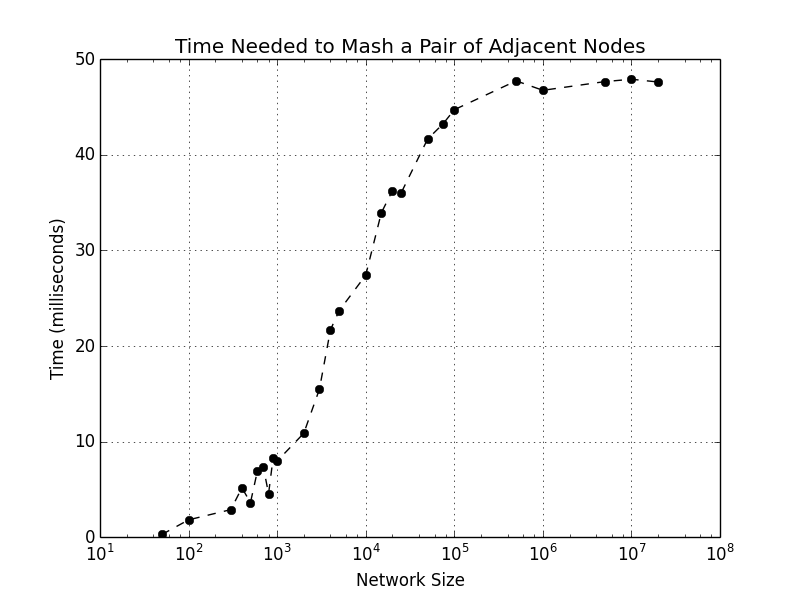
\includegraphics[width=\linewidth]{size_time}
\caption{This figure shows the amount of time needed for an adversary with a single IP address to mash a pair of adjacent nodes.  The time it takes to mash a pair of nodes begins to markedly increase once the network size gets above 1000 until it asymptotes at 48 ms.  For larger networks, more IP addresses are needed and precomputing becomes necessary.}
\label{fig:exp1}
\end{figure}


%TODO REMOVE DECIMALS
\begin{table}\small
    \centering
    \caption{Times and success rate for mashing adjacent nodes for a single IP.}
    \label{tab:exp1}
\begin{tabular}{|r|r|r|}
    \hline
    Network Size &  Success Rate &  Avg Time to Mash (ms) \\ \hline
    50 & 1.0 & 0.29 \\ \hline
    100.0 & 1.0 & 1.82 \\ \hline
    300.0 & 0.99 & 2.89 \\ \hline
    400.0 & 0.98 & 5.16999 \\ \hline
    500.0 & 1.0 & 3.62999 \\ \hline
    600.0 & 0.98 & 6.97 \\ \hline
    700.0 & 0.94 & 7.32 \\ \hline
    800.0 & 0.99 & 4.54999 \\ \hline
    900.0 & 0.92 & 8.28 \\ \hline
    1000.0 & 0.92 & 7.96999 \\ \hline
    2000.0 & 0.95 & 10.88 \\ \hline
    3000.0 & 0.88 & 15.47999 \\ \hline
    4000.0 & 0.74 & 21.7 \\ \hline
    5000.0 & 0.71 & 23.68 \\ \hline
    10000.0 & 0.67 & 27.41 \\ \hline
    15000.0 & 0.5 & 33.93 \\ \hline
    20000.0 & 0.37 & 36.24999 \\ \hline
    25000.0 & 0.39 & 35.98 \\ \hline
    50000.0 & 0.23 & 41.64999 \\ \hline
    75000.0 & 0.2 & 43.25999 \\ \hline
    100000.0 & 0.13 & 44.71999 \\ \hline
    500000.0 & 0.04 & 47.73999 \\ \hline
    1000000.0 & 0.03 & 46.75 \\ \hline
    5000000.0 & 0.0 & 47.65999 \\ \hline
    10000000.0 & 0.0 & 47.90999 \\ \hline
    20000000.0 & 0.0 & 47.62 \\ \hline
    
\end{tabular}
\end{table}
These figures show that the larger the network size, the longer it takes for the adversary to mash a given pair of adjacent nodes.
Eventually, the time it takes to mash a region asymptotes to about 48 milliseconds.
This is the amount of time it takes for the adversary with a single IP to generate all 16383 hash combinations.
While this is a short time to mash a single region, an adversary following the attack specified in our next experiment will want to mash $n-1$ regions.
If the network size is 1 million, this process can take upwards of 13 hours in computational time.

Since the attacker's IP addresses and ports do not change over the course of the attack, the attacker would waste time by generating the same keys over and over. 
The mashing process could also take substantially longer if the network a hash function that produces numbers larger than 160 bits or if the network uses a more expensive function such as scrypt \cite{scrypt}.

The attacker can instead perform all the work needed to mash a network upfront, precomputing all possible valid hash keys.
We have shown this takes about 48 milliseconds for 16383 keys.
Storing these values in a sorted list costs 160 bits for each SHA1 key and 16 bits for each port, for a total of $176  \cdot 16383 = 2,883,408$ bits, or roughly 352 kilobytes for each IP address the attacker has.\footnote{Storing the IP address is unnecessary since it is always the same.}




%check chord coverage just with the successors
\subsection{Experiment 2:  Nearest Neighbor Eclipse via Sybil} %formerly 2
\label{sec:exp2}
The objective of this experiment is to completely eclipse a network using a Sybil attack, starting with a single malicious node.
With simulate this by creating a network of $n$ nodes.
Each node is represented by a key generated by taking the SHA1 of a random IP/port combination.

The goal of the attacker is to mash as many pairs of adjacent nodes as possible.
We call this the \textit{Nearest Neighbor Eclipse} since the attacker seeks to become the nearest neighbors of each node.

The attacker is given $num\_ips$ randomly generated IP addresses, but can use any port between 49152 and 65535.
This gives the attacker $ 16383 \cdot num\_ips $ possible hash keys to use for Sybils.
As mentioned previously in Section \ref{sec:exp1}, the attacker can easily precompute all of theses hash keys and store them in a sorted list to be used as needed, requiring only 352 kilobytes per IP.
Since this list is sorted and this attack will go in order through the network, searching for a key that mashes a pair of nodes takes constant time.

To perform the attack, an adversary choses any random hash key as a starting point to ``join'' the network.
This is his first Sybil and the join process provides information about a number of other nodes.
Most importantly, nodes provide information about other nodes that are close to it, which are provided to ensure fault tolerance between immediate neighbors.
The adversary uses this information to inject Sybils in between successive healthy nodes.
%TODO EXACT FAULT TOLERANCE NUMBERS

For clarity we present this example. 
Consider the small segment of the network made up of adjacent nodes $a$, $b$, $c$, and $d$.
The Sybil joins between nodes $a$ and $b$, and the joining process informs the adversary about node $c$, possibly node $d$, and a handful of other nodes in the network.
The adversary will always learn about node $c$ because a node between $a$ and $b$ would need to know about node $c$ for fault tolerance.

The adversary's next move would be to inject a node between nodes $b$ and $c$.
This is done by selecting a hash key $k$.
The adversary injects a Sybil node with key $k$, which joins in between $b$ and $c$, and the joining process informs the adversary about node $d$ and several other nodes, including many close nodes.
The adversary then aims to inject a node in between $c$ and $d$, and continues \textit{ad nauseam}.  %or ad infitum

Depending on the network size and the number of keys available to the adversary, it is entirely possible the adversary will not have a key to inject between a pair of successive nodes.
In this case, the adversary moves on to the next successive pair that the adversary has learned about.

We simulated this attack on networks of up to 20 million nodes.
We chose 20 million since it falls neatly into the 15-27 million user range seen on Mainline DHT \cite{mainlineMeasure}.
We gave the attacker access to up to 19 IP addresses.
Our results are in Figures \ref{fig:exp2} and \ref{fig:size_prob_all} and Table \ref{tab:exp2}.
For Table \ref{tab:exp2}, we have included only the results for larger sized networks, as the smaller sized networks were completely occluded.


\begin{figure}
\centering
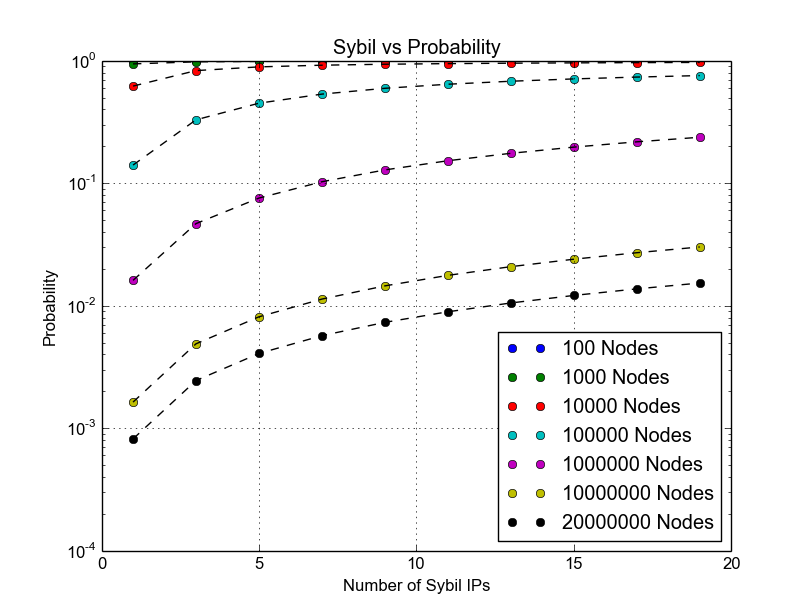
\includegraphics[width=1\linewidth]{ip_prob_all}
\caption[foo]{Our simulation results.  
    The $x$-axis corresponds to the number of IP addresses the adversary can bring to bear.
    The $y$-axis is the probability that a random pair of adjacent nodes can be mashed.
    Each line maps to a different network size of $n$.
    The dotted line traces the line corresponding to the Equation \ref{eq:bad}: $ P_{bad\_neighbor} =  \frac{num\_ips \cdot 16383}{num\_ips \cdot 16383 + n - 1}$}
\label{fig:exp2}
\end{figure}


\begin{figure}
\centering
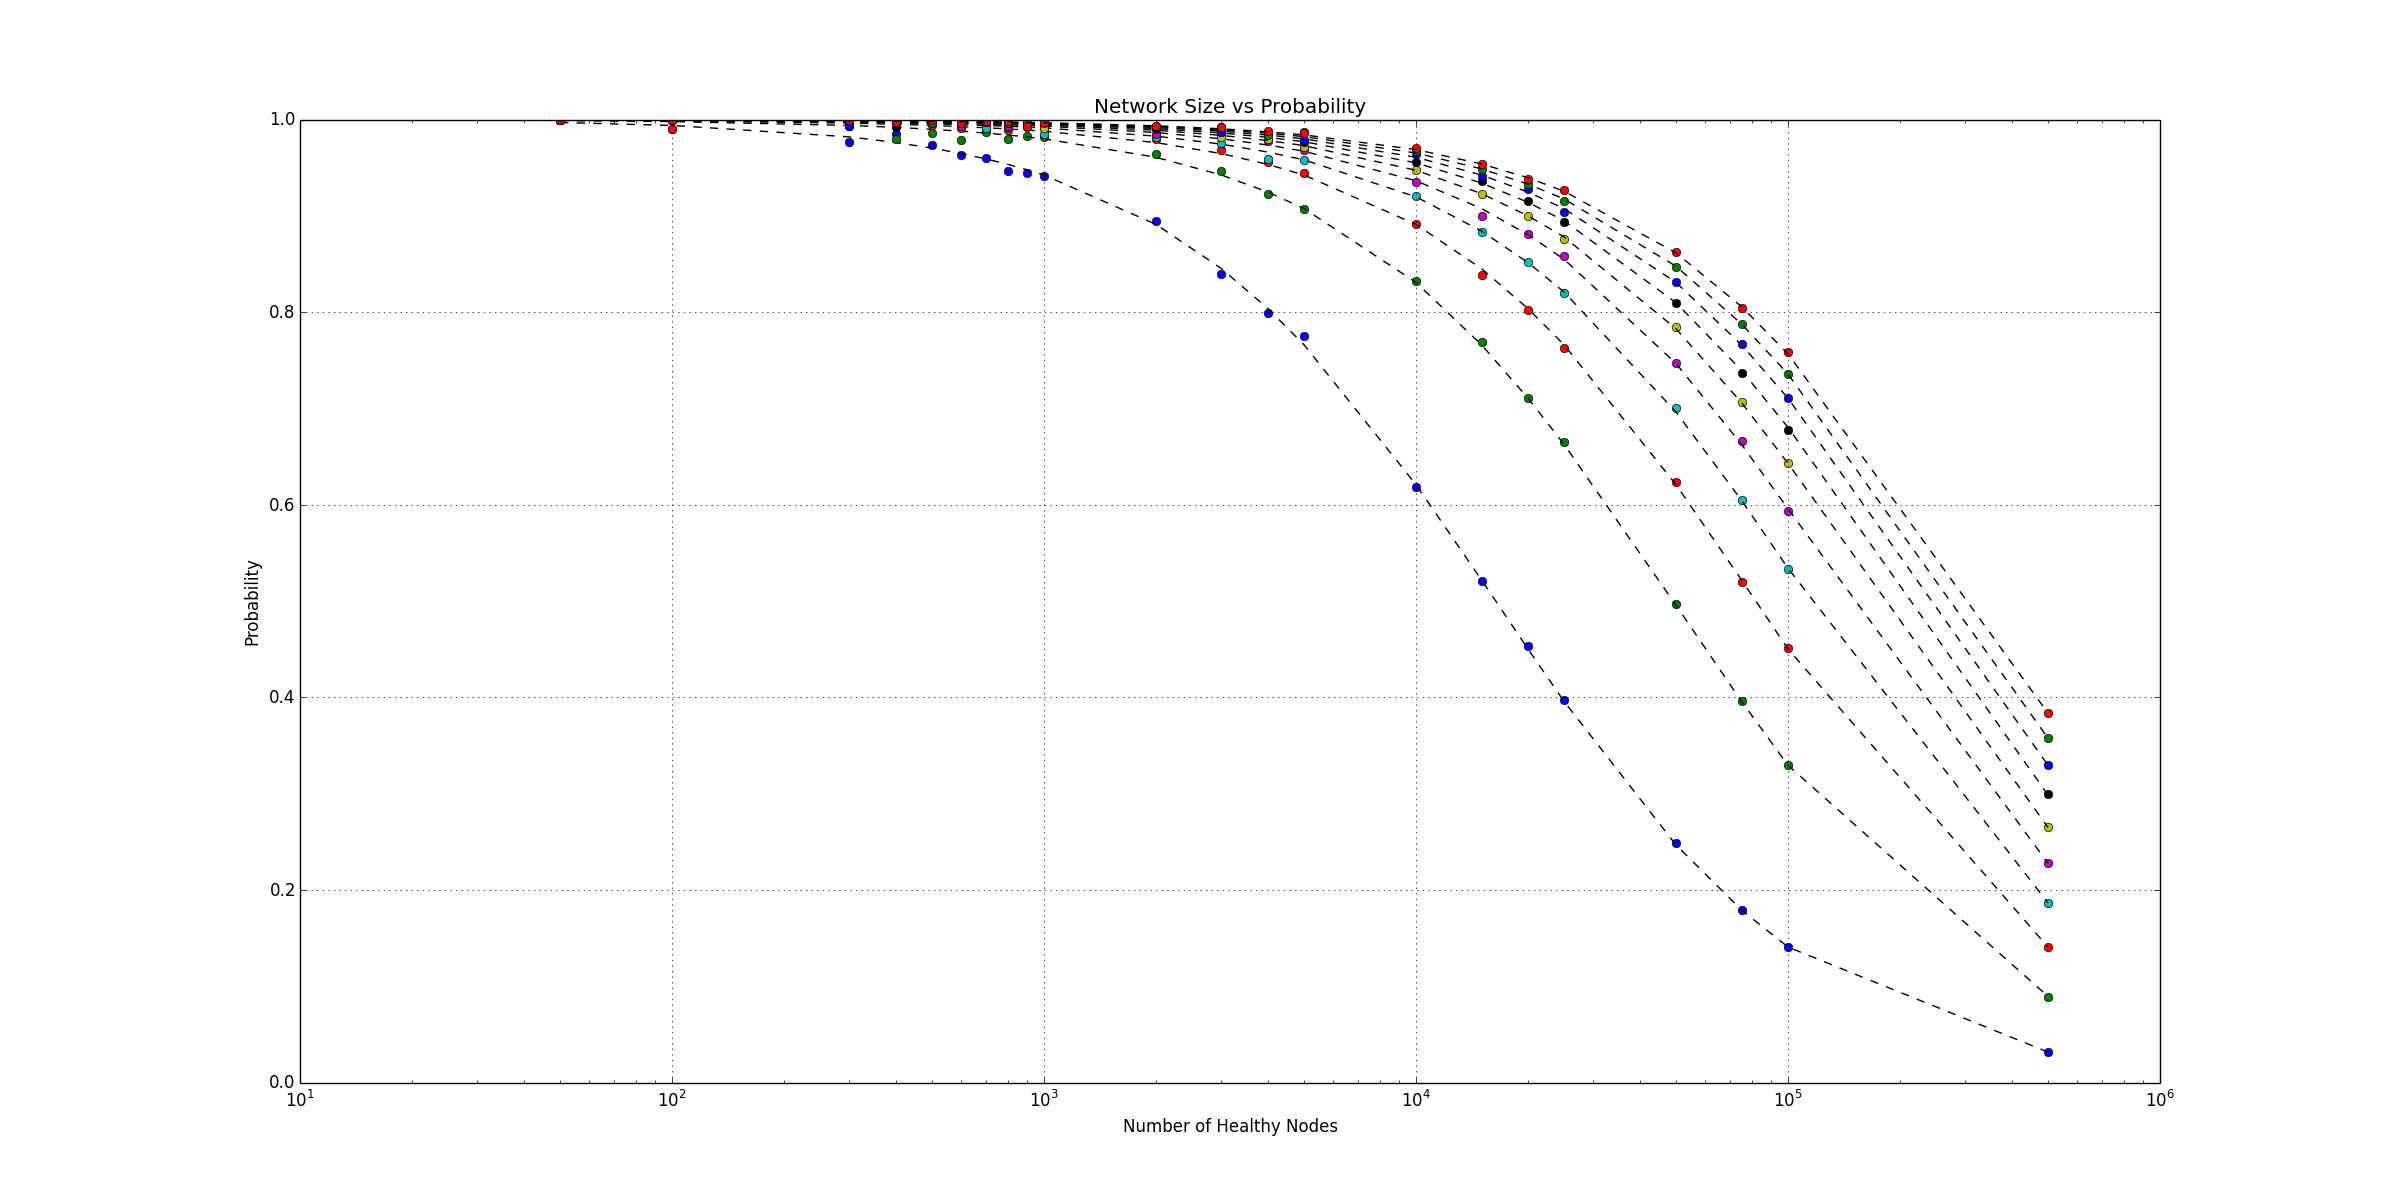
\includegraphics[width=\linewidth]{size_prob_all}
\caption[a]{These are the same as results shown in Figure \ref{fig:exp2}, but our $x$-axis is the network size $n$ in this case.  
    Here, each line corresponds to a different number of unique IP addresses the adversary has at their disposal.}
\label{fig:size_prob_all}
\end{figure}



\begin{table}\small
	\centering
       \caption{Selection of results for Nearest Neighbor Eclipse.}  %The Fraction of regions injected is the percentage of all regions for which the adversary could inject a Sybil with the suitable key. The Sybil/Region measure is how many Sybils were available to inject a particular region on average.}
       \label{tab:exp2}
\begin{tabular}{|r|r|r|r|}
    \hline
    IPs & Network Size &  Success Rate & Sybils/Region \\ \hline
1 & 5000.0 & 0.7748 & 3.2762 \\ \hline
1 & 5000000.0 & 0.0032654 & 0.0032768 \\ \hline
1& 10000000.0 & 0.0016364 & 0.0016384 \\ \hline
1 & 20000000.0 & 0.00081865 & 0.0008192 \\ \hline
5 & 5000.0 & 0.9444 & 16.381 \\ \hline
5 & 5000000.0 & 0.0161208 & 0.016384 \\ \hline
5 & 10000000.0 & 0.0081223 & 0.008192 \\ \hline
5 & 20000000.0 & 0.0040801 & 0.004096 \\ \hline
11 & 5000.0 & 0.9708 & 36.0428 \\ \hline
11 & 5000000.0 & 0.0347646 & 0.0360448 \\ \hline
11 & 10000000.0 & 0.0177117 & 0.0180224 \\ \hline
11 & 20000000.0 & 0.008932 & 0.0090112 \\ \hline
19 & 5000.0 & 0.9834 & 62.2452 \\ \hline
19 & 5000000.0 & 0.058562 & 0.0622592 \\ \hline
19 & 10000000.0 & 0.0301911 & 0.0311296 \\ \hline
19 & 20000000.0 & 0.01532465 & 0.0155648 \\ \hline
\end{tabular}


\end{table}

%NEED TO TEST TO SEE WHAT NEEDED TO ATTACK 50,000,000 size network, twice the size of the BitTorrent network.  CAN WE?
%Each experiment took less than a second to perform.
Our results show that an adversary, given only modest resources, can inject a Sybil in between the vast majority of successive nodes in moderately sized networks.
In a large network, modest resources still can be used to compromise more that a third of the network, an  important goal if the adversary  wishes to launch a Byzantine attack.

Our results match values predicted by Equation \ref{eq:bad}.
However, this experiment only covers the short links of the network, but not the long distance links.

% PLOT for LD50 values for IPS vs Network Size



\subsection{Experiment 3: Fully Complete Eclipse via Sybil}
\label{sec:chord}
We extended the previous experiment by considering the long-distance hops of each node in addition to the short-range links of the DHT.
We choose to model an attack on a P2P system built using Chord \cite{chord}.


We chose to model Chord for a number of reasons.
Chord is an extremely well understood DHT and is very simple to evaluate using simulations.
Nodes in Chord generates long distance links independent of information provided by other nodes, rather than directly querying neighbors.
This minimizes the opportunities adversaries have to poison the node's routing table via false advertisements, which can be on other DHTs such as Pastry \cite{pastry}. 
This makes the Sybil attack the most straightforward means of effecting an Eclipse attack on a Chord network.

Nodes in Chord have $m$ long-range links, one for each of the bits in the keys, which is 160 in our experiments.
Each of node $a$'s long-range links points to the node with the lowest key $\geq a + 2^{i} \mod 2^{m}, 0 \leq i \leq 160$.

However, many of the fingers are redundant and point to the nearest neighbor.
As we have mentioned, on average, nodes are $\frac{2^{m}}{n}$ distance apart.
The smaller the network, the further apart nodes are, and therefore each  node has more redundant fingers and is easier to attack.

The attack is very similar to the Nearest Neighbor attack demonstrated above.
Beside injecting a node in between successive nodes, the attacker also attempts to place a Sybil in between each of the long-range links.
We simulated this attack under the same parameters as above and are presented in Table \ref{tab:exp3}.


\begin{figure}
    \centering
    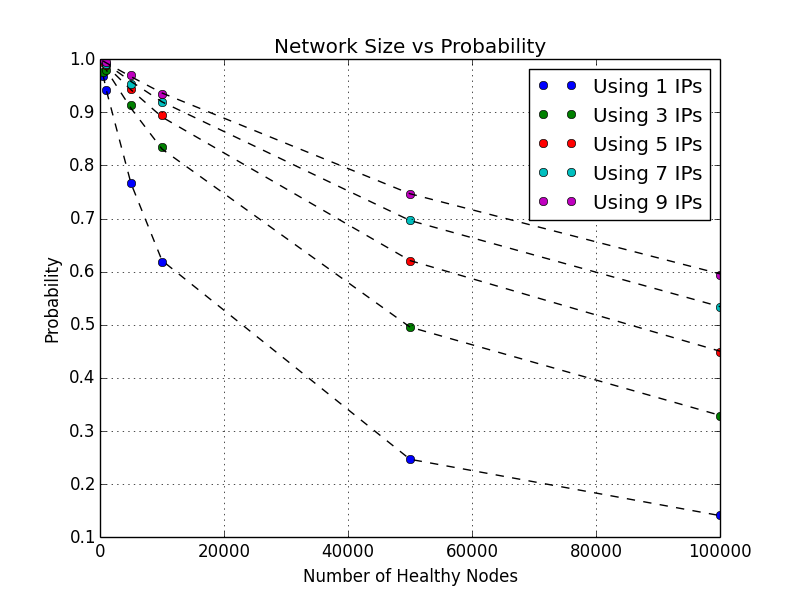
\includegraphics[width=\linewidth]{size_occlusion_chord}
    \caption{This graph shows the relationship between the network size and the probability a particular link in Chord, adjacent or not, can be mashed.
        The dotted line traces the line corresponding to the Equation \ref{eq:bad}: $ P_{bad\_neighbor} =  \frac{num\_ips \cdot 16383}{num\_ips \cdot 16383 + n - 1}$}
    
    \label{fig:exp3}
\end{figure}



\begin{table}\small
    
        \caption{Selection of results for a Sybil attack on Chord.} % The percentage of links occluded is the percentage of long range links from healthy nodes that connect to Sybil nodes. 
            %The Occlusion per node measures how many of the 160 long range links lead to a Sybil on average.  
            %We ignore the predecessor links since it is not used for routing.}
        \label{tab:exp3}
        
        \begin{tabular}{|r|r|r|r|}
            \hline 
            IPs & Network Size &   Success Rate & Occlusions/Node \\ \hline
            1 & 1000 & 0.94186875 & 150.699 \\ \hline
            1 & 10000 & 0.618480625 & 98.9569 \\ \hline
            1 & 100000 & 0.141753625 & 22.68058 \\ \hline
            3 & 1000 & 0.97915625 & 156.665 \\ \hline
            3 & 10000 & 0.83425 & 133.48 \\ \hline
            3 & 100000 & 0.3286290625 & 52.58065 \\ \hline
            5 & 1000 & 0.988725 & 158.196 \\ \hline
            5 & 10000 & 0.894415 & 143.1064 \\ \hline
            5 & 100000 & 0.4488916875 & 71.82267 \\ \hline
            7 & 1000 & 0.99091875 & 158.547 \\ \hline
            7 & 10000 & 0.919071875 & 147.0515 \\ \hline
            7 & 100000 & 0.5337635625 & 85.40217 \\ \hline
            9 & 1000 & 0.9948125 & 159.17 \\ \hline
            9 & 10000 & 0.935495625 & 149.6793 \\ \hline
            9 & 100000 & 0.5936118125 & 94.97789 \\ \hline
            
            
        \end{tabular}
        
        
    
\end{table}





Surprisingly, the percentage of links from healthy nodes that connect to Sybil nodes follows Equation \ref{eq:bad} and the results from \ref{sec:exp2}.
This means performing a Nearest Neighbor Eclipse provides the same results as actively blocking all the long range links in the network.

Our results show that an attacker needs only to focus their efforts on compromising the links between adjacent nodes to attack all the links in the network.


We can calculate that the number of IP addresses needed to compromise half the links in a 20,000,000 node network is 1221 1P addresses.
While this seems like a daunting number of IP addresses, cloud computing has made solutions for an attacker much more accessible and affordable to attackers.
At the time of writing, it would cost \$43.26 USD to use 1221 instances for an hour on Amazon's Elastic Cloud Compute service.
In fact, one of the attacker launching a Sybil attack was identified as having an IP address associated with Amazon's Elastic Cloud Compute \cite{sybilbit}.


%\subsubsection{Plaxton Based networks}


%\section{Masking the Attack}
%Now that we have established that a Sybil attack can be performed with great ease, our focus now turns to avoiding detection.
%The only surefire way to achieve this is by preventing a node from seeing 
%We need a different IP for each point surrounding our victim.  In the Nearest-Neighbor attack, we need a 

%We can reduce this into an interesting graph coloring problem.


%The hard maximum, in general, is $m$ separate IP addresses, one for each bit in a $\log n$ routing/routing table DHT.
%Recall that the vast

\section{Conclusions and Future Work}
%\section{Simple Load Balancing Injection Framework}
\label{sec:horror}

Our analysis and experiments show that an adversary with a small number of machines and limiting their port usage to just the ephemeral ports can easily compromise a P2P system and mash the majority of the regions between nodes.
This effectively prevents nodes from talking to one another without first sending messages through Sybils, who can eavesdrop on them or disregard the eaves and move straight on to the dropping.

Our discussion have primarily concerned Chord, but an astute reader may wonder why did we not simulate an attack on Mainline DHT  \cite{mainline}, the Kademlia \cite{kademlia} based DHT used as the backend of BitTorrent.
It is ostensibly the largest P2P system in use, so it seems more suited for analyzing our mash-based attack than Chord.

We avoided simulating the mashing process on MLDHT because, as we noted earlier in Section \ref{sec:assume}, it is completely unnecessary to perform any mashing.
In MLDHT, a node ID is not chosen by hashing an IP and port combination, but by picking an address uniformly at random between 0 and $2^{160}-1$.

An adversary who wants to a completely isolate a node on the network can choose Sybils with ``random'' hashkeys completely eliminate that node from the routing tables of healthy peers. 
Research has examined MLDHT's vulnerability to Sybil attacks \cite{sybilbit} and detected entities performing the attack on MLDHT.
Our research demonstrates that switching to using a SHA1 hash of the IP and port is no defense against a Sybil attack, since the adversary can easily mash into appropriate places.
%A big difference is their honeypots target those who respond to everything.




However, the mashing process can be used in non-security related settings to benefit a DHT.
As we have mention previously, the SHA1 hash has an evenly distributed output, but no set of keys will be completely evenly distributed.
Some nodes will be responsible for larger regions than others and therefore be responsible for a larger portion for the work.

If a node can detect a when a peer has too much of a load, the node can inject a virtual node into the region to shoulder some of the load.
Too much of a load could be defined by having a too large region or by watching traffic requests.
This could be integrated into a distributed key allocation system, so that a node can bind these keys to itself, but only use a small portion of the keys alloted to it to aid with load-balancing.
The only cost would be that node would have to keep track of the keys it can inject, which we mentioned was only 320 kilobytes of data.

\bibliographystyle{IEEEtran}
\bibliography{potato}

\end{document}
